\section{作业2}
\subsection{作业2.1}
\subsubsection{题目描述}

令文法为

\begin{align*}
E &\rightarrow E \vee T\;|\;T\\
T &\rightarrow T \wedge F\;|\; F\\
F &\rightarrow \neg F\;|\;(E)\;|\; i
\end{align*}

\begin{enumerate}
    \item 写出 $i \wedge(E)$  的最左推导和最右推导。
    \item 画出 $i_{1} \wedge \neg\left(i_{2} \vee i_{3}\right)$ 的语法树。
    \item 写出 $i_{1} \wedge \neg\left(i_{2} \vee i_{3}\right)$ 的所有短语、直接短语和句柄
\end{enumerate}

\subsubsection{解答}

\paragraph{题目 2.1.1} 若推导过程中,总是最先替换最右(左)的非终结符,则称为最右(左)推导:

\begin{align*}
E & \Rightarrow {\color{Green} T} \Rightarrow {\color{Green} T} \wedge F \Rightarrow {\color{Green} F}  \wedge F  \Rightarrow i \wedge {\color{Green} F}  \Rightarrow i \wedge (E) \\
E & \Rightarrow {\color{Green} T} \Rightarrow T \wedge {\color{Green} F} \Rightarrow {\color{Green} T}  \wedge (E) \Rightarrow {\color{Green} F}   \wedge (E) \Rightarrow i \wedge (E)
\end{align*}

\paragraph{题目 2.1.2} 首先写出一个推导:

\[
{\color{EE} E} \Rightarrow {\color{TT} T} \Rightarrow {\color{TT} T}{\color{oo} \wedge} {\color{FF} F} \Rightarrow {\color{FF} F}{\color{oo} \wedge\neg} {\color{FF} F} \Rightarrow {\color{oo}i_1}{\color{oo} \wedge\neg(}{\color{EE} E}{\color{oo} )} \Rightarrow {\color{oo}i_1}{\color{oo} \wedge\neg(}{\color{EE} E}\vee {\color{TT} T}{\color{oo} )} \overset {...} \Longrightarrow {\color{oo}i_1}{\color{oo} \wedge\neg (}{\color{oo}i_2} \vee {\color{oo}i_3}{\color{oo} )}
\]

于是可以画出语法树:

\begin{center} 
\begin{tikzpicture}[
  level distance=10mm, % 调整上下两行的间隔
  level 1/.style={sibling distance=40mm},
  level 2/.style={sibling distance=30mm},
  level 3/.style={sibling distance=25mm},
  level 4/.style={sibling distance=15mm},
  level 5/.style={sibling distance=10mm},
  every node/.style={draw, circle, minimum size=7mm, inner sep=2pt},
  colorE/.style={draw=EE},
  colorT/.style={draw=TT},
  colorF/.style={draw=FF},
  coloro/.style={draw=oo},
  ]

% Root node
\node[colorE]{$E$}
  child { node[colorT]{$T$}
    child { node[colorT]{$T$}
        child { node[colorF]{$F$}
            child { node[coloro]{$i_1$} }
        }
    }
    child { node[coloro]{$\wedge$} }
    child { node[colorF]{$F$} 
        child { node[coloro]{$\neg$} }
        child { node[colorF]{$F$}
            child { node[coloro]{$($} }
            child { node[colorE]{$E$}
                child { node[colorE]{$E$}
                    child { node[colorT]{$T$}
                        child { node[colorF]{$F$}
                            child { node[coloro]{$i_2$} }
                        }
                    }
                }
                child { node[coloro]{$\vee$} }
                child { node[colorT]{$T$}
                    child { node[colorF]{$F$}
                        child { node[coloro]{$i_3$} }
                    }
                }
            }
            child { node[coloro]{$)$} }
        }
    }
  };

\end{tikzpicture}
\end{center} 

\paragraph{题目 2.1.3} 由于(3)与(2)的语句相同,于是可以看图说话:

\begin{enumerate}
    \item 短语:$i_{1} \wedge \neg\left(i_{2} \vee i_{3}\right)$、$i_1$、$\wedge$、$\neg\left(i_{2} \vee i_{3}\right)$、$\left(i_{2} \vee i_{3}\right)$、$i_{2} \vee i_{3}$、$i_{2}$、$\vee$、$i_{3}$;
    \item 直接短语:$i_1$、$i_2$、$i_3$;
    \item 句柄:$i_1$。
\end{enumerate}


\subsection{作业2.2}
\subsubsection{题目描述}
证明下面的文法是二义的:$S\rightarrow iSeS\;|\;iS\;|\;i$
\subsubsection{解答}
和if-else长得差不多,类似课件中的上下文无关文法表示条件语句,可以采用两个 $i$ 对应一个 $e$ 的方式来构造,也就是 $iiSeS$ 这种形式:

\begin{itemize}
    \item $S\Rightarrow {\color{Red} iS} \Rightarrow {\color{Red} i} {\color{Blue} iSeS} $;
    \item $S\Rightarrow {\color{Blue} iSeS } \Rightarrow {\color{Blue} i} {\color{Red} iS} {\color{Blue} eS} $。
\end{itemize}

右侧以 $iiiei$ 为例子画出不同的语法树:
\vspace{5mm}
\begin{center}
\begin{tikzpicture}
    \begin{tikzpicture}[
      level distance=10mm, 
      level 1/.style={sibling distance=15mm},
      level 2/.style={sibling distance=10mm},
      every node/.style={draw, circle, minimum size=7mm, inner sep=2pt},
      color1/.style={draw=red},
      color2/.style={draw=blue}
    ]
    \node {$S$}
        child { node[color1]{$i$} }
        child { node[color1]{$S$}
            child { node[color2]{$i$} }
            child { node[color2]{$S$}
                child { node[color2]{$i$} }
            }
            child { node[color2]{$e$} }
            child { node[color2]{$S$}
                child { node[color2]{$i$} }
            }
        }
    ;
    \end{tikzpicture}
    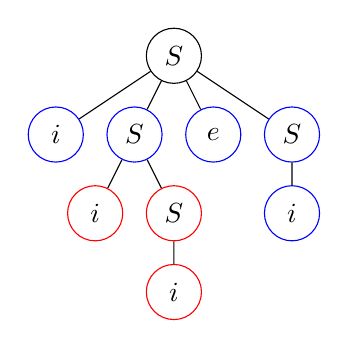
\begin{tikzpicture}[
      level distance=10mm, 
      level 1/.style={sibling distance=10mm},
      level 2/.style={sibling distance=10mm},
      every node/.style={draw, circle, minimum size=7mm, inner sep=2pt},
      color1/.style={draw=red},
      color2/.style={draw=blue}
    ]
    \node {$S$}
        child { node[color2]{$i$} }
        child { node[color2]{$S$}
            child { node[color1]{$i$} }
            child { node[color1]{$S$}
                child { node[color1]{$i$} }
            }
        }
        child { node[color2]{$e$} }
        child { node[color2]{$S$}
            child { node[color2]{$i$} }
        }
    ;
    \end{tikzpicture}
\end{tikzpicture}
\end{center}
\vspace{-40mm}
\subsection{作业2.3}
\subsubsection{题目描述}
类Lisp 程序文法
\begin{align*}
    G[E]:\;\; &E \rightarrow(A, E, E)\;|\;i\\
    &A \rightarrow+\;|\;-\;|\;\times\;|\;{\div}
\end{align*}
\begin{enumerate}
\item 任意变量与  $i$  匹配,  $(\theta, a, b)$  表示  $a \theta b$  的结果,其中  $\theta$  为运算符,试写出  $a \times(b+c)  {\div} d$  的类Lisp 程序形式;
\item 画出上述句子的语法树;
\item 写出上述句子的短语、直接短语和句柄。
\end{enumerate}
\subsubsection{解答}

\paragraph{题目2.3.1} 首先不难画出 $a \times(b+c)  {\div} d$ 的表达式树:


\begin{center} 
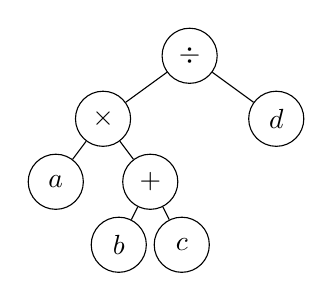
\begin{tikzpicture}[
  level distance=8mm, % 调整上下两行的间隔
  level 1/.style={sibling distance=22mm},
  level 2/.style={sibling distance=12mm},
  level 3/.style={sibling distance=8mm},
  every node/.style={draw, circle, minimum size=7mm, inner sep=2pt},
  ]

% Root node
\node{${\div}$}
    child { node{$\times$}
        child { node{$a$} }
        child { node{$+$}
            child { node{$b$} }
            child { node{$c$} }
        }
    }
    child { node{$d$} };

\end{tikzpicture}
\end{center} 

于是可以写出类Lisp程序形式(实际上是前序遍历的形式?)为:$({\div},(\times,a,(+,b,c)),d)$。

\paragraph{题目2.3.2} 根据上面的程序形式可以写出推导过程:

\begin{align*}
E & \Rightarrow (A,E,E)\\
& \Rightarrow (\div, (A,E,E), d)\\
& \Rightarrow (\div, (\times, a, (A,E,E)), d) \\
& \Rightarrow (\div, (\times, a, (+,b,c)), d)
\end{align*}

不难画出语法树:

\begin{center} 
\begin{tikzpicture}[
  level distance=20mm, % 调整上下两行的间隔
  level 1/.style={sibling distance=23mm},
  level 2/.style={sibling distance=13mm},
  level 3/.style={sibling distance=6mm},
  every node/.style={draw, circle, minimum size=5.5mm, inner sep=1pt},
  NodeE/.style={draw=EE},
  NodeA/.style={draw=TT},
  leaf1/.style={draw=FF},
  leaf2/.style={draw=oo},
  ]


\node[NodeE]{$E$}
    child { node[leaf1]{$($} }
    child { node[NodeA]{$A$}
        child { node[leaf2]{$\div$} }
    }
    child { node[leaf1]{$,$} }
    child { node[NodeE]{$E$}
        child { node[leaf1]{$($} }
        child { node[NodeA]{$A$}
            child { node[leaf2]{$\times$} }
        }
        child { node[leaf1]{$,$} }
        child { node[NodeE]{$E$}
            child { node[leaf2]{$a$} }
        }
        child { node[leaf1]{$,$} }
        child { node[NodeE]{$E$}
            child { node[leaf1]{$($} }
            child { node[NodeA]{$A$}
                child { node[leaf2]{$+$} }
            }
            child { node[leaf1]{$,$} }
            child { node[NodeE]{$E$}
                child { node[leaf2]{$b$} }
            }
            child { node[leaf1]{$,$} }
            child { node[NodeE]{$E$}
                child { node[leaf2]{$c$} }
            }
            child { node[leaf1]{$)$} }
        }
        child { node[leaf1]{$)$} }
    }
    child { node[leaf1]{$,$} }
    child { node[NodeE]{$E$}
        child { node[leaf2]{$d$} }
    }
    child { node[leaf1]{$)$} };

\end{tikzpicture}
\end{center} 

\paragraph{题目2.3.3} 根据上图看图写话:

\begin{enumerate}
    \item 短语:$\color{TT}({\div},(\times,a,(+,b,c)),d)$、$\color{FF}($、$\color{oo}{\div}$、$\color{FF},$、$\color{TT}(\times,a,(+,b,c))$、$\color{oo}d$、$\color{FF})$、$\color{oo}\times$、$\color{oo}a$、$\color{TT}(+,b,c)$、$\color{oo}+$、$\color{oo}b$、$\color{oo}c$;
    \item 直接短语:$\color{oo}\div$、$\color{oo}\times$、$\color{oo}a$、$\color{oo}+$、$\color{oo}b$、$\color{oo}c$、$\color{oo}d$;
    \item 句柄:$\color{oo}\div$。
\end{enumerate}